\documentclass[]{article}
\usepackage[utf8]{inputenc}
\usepackage[english,russian]{babel}
\usepackage{amsmath}
\usepackage{enumerate}
\usepackage[12pt]{extsizes}
\linespread{1.3}
\usepackage[left=3cm, top=1.5cm, right=1.3cm, bottom=2cm, nohead, footskip=10mm]{geometry}


\usepackage[absolute,overlay]{textpos}
\usepackage{indentfirst}
\usepackage{float}
\restylefloat{table}
\usepackage{hyperref}
\usepackage{mathtext}
\usepackage{amsfonts}
\usepackage{amsthm}
\usepackage{tikz}
\usepackage{xspace}
\usepackage{listings}
\usetikzlibrary{shapes,positioning,shadows,trees,automata,arrows.meta,shapes.geometric}
\usepackage{pgf-pie}
\usepackage{chngcntr}
\usepackage{pdfpages}
\usepackage{systeme}
\usepackage{empheq}
\numberwithin{equation}{section}
\usepackage{caption}
\DeclareCaptionLabelSeparator{none}{. }
\captionsetup{labelsep=none}


\pagestyle{plain}

\renewcommand{\labelenumii}{\theenumii}
\renewcommand{\theenumii}{\arabic{enumii}.}

\captionsetup[lstlisting]{
    singlelinecheck=false
    ,margin=3pt,
    font=,
    skip=5pt
    }


\lstdefinestyle{TEXTstyle}{
    basicstyle=\footnotesize\ttfamily,
    aboveskip=0pt,
	belowskip=10pt,
	showspaces=false,
	showstringspaces=false,
    basicstyle=\ttfamily\footnotesize,
    texcl=true,
    morecomment=[l]{\#},
    commentstyle=\color{gray},
    frame=tb
}

\begin{document}
    \thispagestyle{empty}
	\begin{center}
		Министерство образования и науки Российской Федерации\\
		Санкт-Петербургский государственный технический университет\\
		Институт прикладной математики и механики\\
		Кафедра <<Телематика>>\\
		\vspace{5cm}
		\textbf{\textbf{ЛАБОРАТОРНАЯ РАБОТА}}\\
        \vspace{0.5cm}
        \textbf{ПО ТЕМЕ}\\
        \vspace{0.5cm}
		\textbf{\textbf{<<Регрессионные алгоритмы>>}}\\
		\vspace{3cm}
		по направлению 02.04.01.02 <<Организация и управление суперкомпьютерными системами>>
	\end{center}
	\vspace{2cm}
	\begin{tabular} {l l l}
	\hspace{9.5cm} & Выполнил: & \\
	& Студент гр. 13643.1 & Титов А.И.\\
	& Проверил: & Уткин Л.В.
	\end{tabular}
	\vspace{4.5cm}
	\begin{center}
		Санкт-Петербург\\
		2019
    \end{center}


	\renewcommand\contentsname{Оглавление}
	\tableofcontents

    \newpage
    \section*{Постановка задачи}
    \addcontentsline{toc}{section}{Постановка задачи}

    \begin{enumerate}
        \item Загрузите данные из файла <<reglab1.txt>>. Используя функцию lm, постройте регрессию (используйте разные модели). Выберите наиболее подходящую модель, объясните свой выбор.
        \item Реализуйте следующий алгоритм для уменьшения количества признаков, используемых для построения регрессии: для каждого $k \in {0,..,d}$ выбрать подмножество признаков мощности $k^{l}$, минимизирующее остаточную сумму квадратов RSS. Используя полученный алгоритм, выберите оптимальное подможество признаков для данных из файла <<reglab2.txt>>. Объясните свой выбор. Для генерации всех возможных сочетаний по m элементов из некоторого множества x можно использовать функцию combn(x, m, ...).
        \item Загрузите данные из файла <<cygage.txt>>. Постройте регрессию, выражающую зависимость возраста исследуемых отложений от глубины залегания, используя веса наблюдений. Оцените качество построенной модели.
        \item Загрузите данные <<Longley>> (макроэкономические данные). Данные состоят из 7 экономических переменных, наблюдаемых с 1947 по 1962 годы (n=16):
            \begin{enumerate}
                \item GNP.deflator - дефлятор цен
                \item GNP - валовой национальный продукт
                \item Unemployed – число безработных
                \item Armed.Forces – число людей в армии
                \item Population – население, возраст которого старше 14 лет
                \item Year - год
                \item Employed – количество занятых
            \end{enumerate}
        Построить регрессию lm(Employed $\sim$ .) .
        Исключите из набора данных <<longley>> переменную <<Population>>. Разделите данные на тестовую и обучающую выборки равных размеров случайным образом. Постройте гребневую регрессию для значений $\lambda = 10^{-3 + 0.2 i}, i = 0,...,25$, подсчитайте ошибку на тестовой и обучающей выборке для данных значений $\lambda$, постройте графики. Объясните полученные результаты.
        \item Загрузите данные EuStockMarkets из пакета <<datasets>>. Данные содержат ежедневные котировки на момент закрытия фондовых бирж: Germany DAX (Ibis), Switzerland SMI, France CAC, и UK FTSE. Постройте на одном графике все кривые изменения котировок во времени. Постройте линейную регрессию для каждой модели в отдельности и для всех моделей вместе. Оцените, какая из бирж имеет наибольшую динамику.
        \item Загрузите данные JohnsonJohnson из пакета <<datasets>>. Данные содержат поквартальную прибыль компании Johnson $\&$ Johnson с 1960 по 1980 гг. Постройте на одном графике все кривые изменения прибыли во времени. Постройте линейную регрессию для каждого квартала в отдельности и для всех кварталов вместе. Оцените, в каком квартале компания имеет наибольшую и наименьшую динамику доходности. Сделайте прогноз по прибыли в 2016 году во всех кварталах и в среднем по году.
        \item Загрузите данные sunspot.year из пакета <<datasets>>. Данные содержат количество солнечных пятен с 1700 по 1988 гг. Постройте на графике кривую изменения числа солнечных пятен во времени. Постройте линейную регрессию для данных.
        \item Загрузите данные из файла пакета «UKgas.scv». Данные содержат объемы ежеквартально потребляемого газа в Великобритании с 1960 по 1986 гг. Постройте линейную регрессию для каждого квартала в отдельности и для всех кварталов вместе. Оцените, в каком квартале потребление газа имеет наибольшую и наименьшую динамику доходности. Сделайте прогноз по потреблению газа в 2016 году во всех кварталах и в среднем по году.
        \item Загрузите данные <<cars>> из пакета <<datasets>>. Данные содержат зависимости тормозного пути автомобиля (футы) от его скорости (мили в час). Данные получены в 1920 г. Постройте регрессионную модель и оцените длину тормозного пути при скорости 40 миль в час.
    \end{enumerate}

    \newpage
    \section{Набор данных <<reglab1>>}

    В рамках задания были построены две модели: линейная регрессия и гребневая регрессия. Гребневая регрессия была рассмотрена с разными параметрами $\lambda$. Для построенных моделей была получена информация, которая позволяет сказать какая из моделей более применима в данной ситуации (Листинг 1-2). Как можно заметить, при значениях $\lambda$ (K) 0.0 и 0.1 полученные результаты близки, но гребневая регрессия достигает немного лучших результатов.

    \begin{lstlisting}[style = TEXTstyle, caption = Сводка по алгоритму линейной регрессии]
Residuals:
     Min       1Q   Median       3Q      Max
-0.97246 -0.16759  0.01308  0.20537  0.81127

Coefficients:
            Estimate Std. Error t value Pr(>|t|)
(Intercept) -0.02163    0.06384  -0.339    0.735
x            4.10248    0.08698  47.168   <2e-16 ***
y            4.94308    0.08035  61.517   <2e-16 ***
---
Signif. codes:  0 '\*\*\*' 0.001 '\*\*' 0.01 '\*' 0.05 '.' 0.1 ' ' 1

Residual standard error: 0.3376 on 197 degrees of freedom
Multiple R-squared:  0.9686,    Adjusted R-squared:  0.9683
F-statistic:  3041 on 2 and 197 DF,  p-value: < 2.2e-16
    \end{lstlisting}

    \begin{lstlisting}[style = TEXTstyle, caption = Сводка по алгоритму гребневой регрессии]
       Variance Bias^2    MSE rsigma2        F     R2 adj-R2     CN
K=0      0.2269 0.0000 0.2269  0.1134 3056.746 0.9686 0.9685 1.0253
K=0.01   0.2231 0.0656 0.2886  0.1138 3047.745 0.9498 0.9495 1.0250
K=0.02   0.2206 0.2573 0.4779  0.1147 3021.722 0.9315 0.9311 1.0248
K=0.03   0.2193 0.5678 0.7872  0.1163 2980.502 0.9137 0.9132 1.0246
K=0.04   0.2191 0.9904 1.2095  0.1185 2926.186 0.8964 0.8959 1.0243
K=0.05   0.2199 1.5185 1.7384  0.1212 2861.028 0.8796 0.8790 1.0241
K=0.06   0.2214 2.1460 2.3675  0.1244 2787.278 0.8632 0.8625 1.0239
K=0.07   0.2237 2.8673 3.0910  0.1281 2707.080 0.8474 0.8466 1.0236
K=0.08   0.2267 3.6767 3.9034  0.1322 2622.398 0.8319 0.8311 1.0234
K=0.09   0.2302 4.5693 4.7995  0.1368 2534.960 0.8169 0.8160 1.0232
K=0.1    0.2343 5.5401 5.7744  0.1417 2446.246 0.8023 0.8013 1.0230
    \end{lstlisting}

    \section{Набор данных <<reglab2>>}

    Для того, чтобы проанализировать зависимость качества построенной модели от используемых признаков был разработан алгоритм, который перебирает всевозможные сочетания признаков, обучает по каждому из них алгоритм линейной регрессии и составляет список полученных значений остаточной суммы квадратов RSS. В результате работы программы выводится отсортированный список (Листинг 3). Рассматривая список можем сделать вывод, что наибольший вклад в работу алгоритма дают признаки <<x1>> и <<x2>>, в то время как <<x3>> и <<x4>> не несут особого смысла в использовании. Таким образом, оптимальным набором признаков для примера будет <<x1 + x2>>.

    \begin{lstlisting}[style = TEXTstyle, caption = Результат работы программы]
          formulas           r2
4           y ~ x4 0.0002156613
3           y ~ x3 0.0030028334
10       y ~ x3+x4 0.0030832553
2           y ~ x2 0.3203386236
9        y ~ x2+x4 0.3214525377
8        y ~ x2+x3 0.3214796027
14    y ~ x2+x3+x4 0.3223763063
1           y ~ x1 0.6016481121
7        y ~ x1+x4 0.6016493980
6        y ~ x1+x3 0.6038415846
13    y ~ x1+x3+x4 0.6038560928
5        y ~ x1+x2 0.9986369522
12    y ~ x1+x2+x4 0.9990828715
11    y ~ x1+x2+x3 0.9991581283
15 y ~ x1+x2+x3+x4 0.9995113366
    \end{lstlisting}

    \section{Набор данных <<cygage>>}

    Была построена регрессия на основе алгоритма линейной регрессии. Для анализа полученной модели была выведена сводка (Листинг 4). По качеству модели имеет смысл выделить весьма высокий показатель RSS = 0.9737, что говорит о хорошем подборе признаков для обучения модели и достаточно низкую относительно значений исходных данных стандартную ошибку = 522.1.

    \newpage
    \begin{lstlisting}[style = TEXTstyle, caption = Сводка по модели линейной регрессии]
Weighted Residuals:
   Min     1Q Median     3Q    Max
-784.6 -137.7  200.8  466.6  702.4

Coefficients:
            Estimate Std. Error t value Pr(>|t|)
(Intercept)  784.570    422.882   1.855   0.0932 .
Depth         21.909      1.139  19.235 3.14e-09 ***
---
Signif. codes:  0 '***' 0.001 '**' 0.01 '*' 0.05 '.' 0.1 ' ' 1

Residual standard error: 522.1 on 10 degrees of freedom
Multiple R-squared:  0.9737,    Adjusted R-squared:  0.9711
F-statistic:   370 on 1 and 10 DF,  p-value: 3.141e-09
    \end{lstlisting}

    \section{Набор данных <<Longley>>}

    Была построена модель гребневой регрессии с заданными значения параметра $\lambda$. Исходная выборка была разбита на тренировочный и тестовый наборы данных. Ниже представлена собранная информация о зависимости качества модели от параметра $\lambda$ (Листинг 5 и Рис. 1).

    \begin{lstlisting}[style = TEXTstyle, caption = Сводка по регрессионым моделям]
        Variance    Bias^2       MSE rsigma2       F     R2  adj-R2      CN
K=0.1     1.8115  946.0791   947.890   0.483  36.395  0.897  0.7612 35.8817
K=0.158   1.3596  960.6121  961.9717  0.5836 30.1782 0.8660  0.6872 23.0497
K=0.251   1.0366  972.4070  973.4436  0.6962 25.2956 0.8212  0.5829 14.9288
K=0.398   0.8378  981.5793  982.4171  0.8409 20.9436 0.7587  0.4369  9.7950
K=0.630   0.7342  988.4988  989.2330  1.0635 16.5601 0.6741  0.2396  6.5518
K=1       0.6887  993.7733  994.4620  1.4407 12.2241 0.5670 -0.0104  4.5040
K=1.584   0.6587  998.0997  998.7584  2.0666  8.5217 0.4433 -0.2990  3.2113
K=2.511   0.5997 1002.0891 1002.6888  3.0073  5.8562 0.3167 -0.5944  2.3954
K=3.981   0.4900 1006.0959 1006.5858  4.2383  4.1552 0.2043 -0.8566  1.8805
K=6.309   0.3483 1010.1273 1010.4756  5.6233  3.1318 0.1188 -1.0562  1.5556
K=10      0.2149 1013.9307 1014.1456  6.9726  2.5258 0.0627 -1.1871  1.3506
K=15.848  0.1172 1017.2122 1017.3294  8.1343  2.1650 0.0305 -1.2621  1.2212
K=25.118  0.0580 1019.8109 1019.8689  9.0424  1.9476 0.0139 -1.3008  1.1396
K=39.810  0.0267 1021.7301 1021.7568  9.7037  1.8149 0.0061 -1.3191  1.0881
K=63.095  0.0117 1023.0759 1023.0876 10.1621  1.7330 0.0026 -1.3273  1.0556
K=100     0.0049 1023.9860 1023.9910 10.4694  1.6822 0.0011 -1.3308  1.0351
K=158.48  0.0020 1024.5867 1024.5887 10.6710  1.6504 0.0004 -1.3323  1.0221
K=251.188 0.0008 1024.9767 1024.9775 10.8014  1.6304 0.0002 -1.3329  1.0140
K=398.107 0.0003 1025.2274 1025.2277 10.8850  1.6179 0.0001 -1.3332  1.0088
K=630.95  0.0001 1025.3874 1025.3875 10.9383  1.6100 0.0000 -1.3333  1.0056
K=1000    0.0001 1025.4891 1025.4891 10.9721  1.6051 0.0000 -1.3333  1.0035
K=1584.8  0.0000 1025.5535 1025.5536 10.9935  1.6020 0.0000 -1.3333  1.0022
K=2511.8  0.0000 1025.5943 1025.5944 11.0071  1.6000 0.0000 -1.3333  1.0014
K=3981.07 0.0000 1025.6201 1025.6201 11.0156  1.5987 0.0000 -1.3333  1.0009
K=6309.57 0.0000 1025.6364 1025.6364 11.0211  1.5979 0.0000 -1.3333  1.0006
K=10000   0.0000 1025.6467 1025.6467 11.0245  1.5975 0.0000 -1.3333  1.0004
    \end{lstlisting}

    \begin{figure}[H]
        \centering
        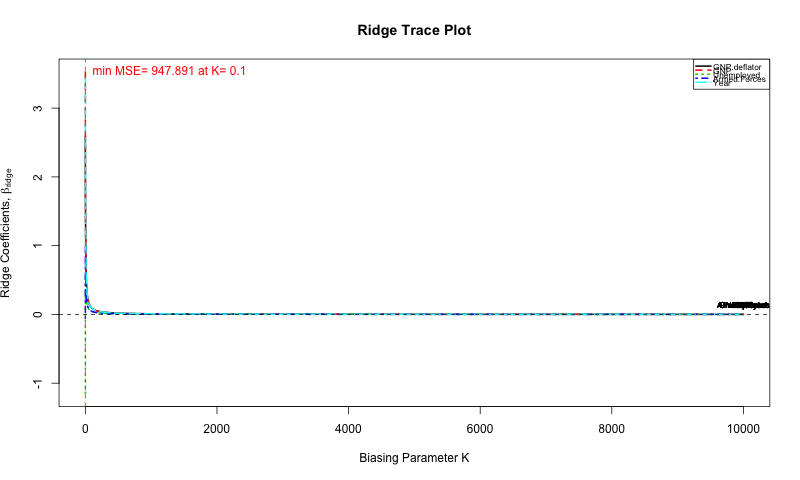
\includegraphics[width = 0.9\linewidth]{data/longley.png}
        \caption{Зависимость качества моделей от параметра $\lambda$}
    \end{figure}

    \section{Набор данных <<EuStockMarkets>>}

    Для того, чтобы изучить набор данных были построенные кривые изменения во времени для всех бирж (Рис. 2).

    \begin{figure}[H]
        \centering
        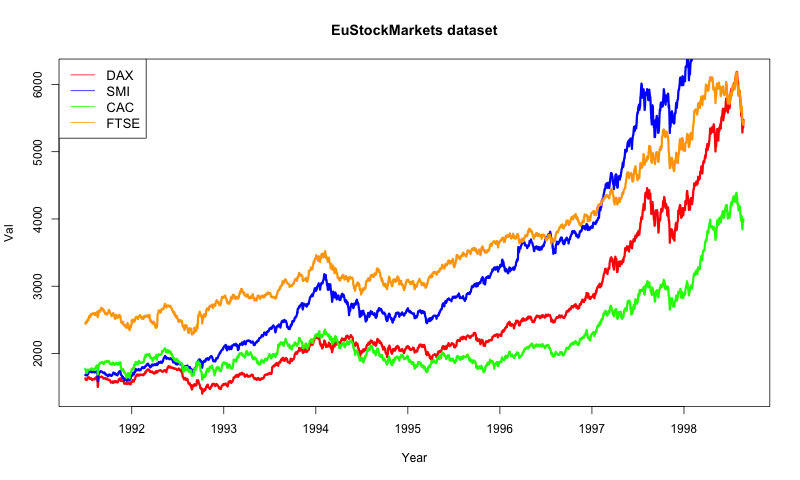
\includegraphics[width = 0.8\linewidth]{data/stcokmark_data.png}
        \vspace{-0.5cm}
        \caption{Набор данных <<EuStockMarkets>>}
    \end{figure}
    \vspace{-0.4cm}
    Были построены модели линейной регрессии для каждой из бридж (Рис. 3).
    \vspace{-0.3cm}
    \begin{figure}[H]
        \centering
        \begin{tabular}{c c}
            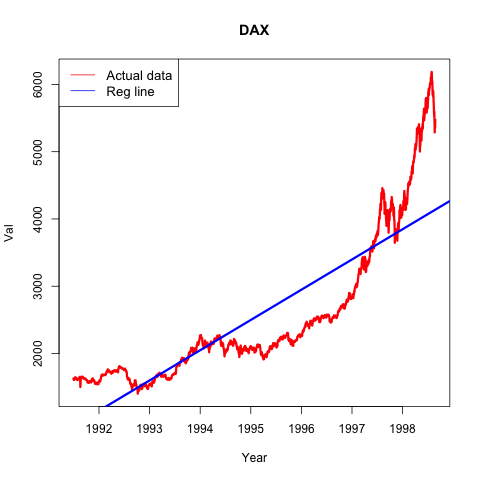
\includegraphics[width = 0.4\linewidth]{data/stockmark_reg_DAX.png} & 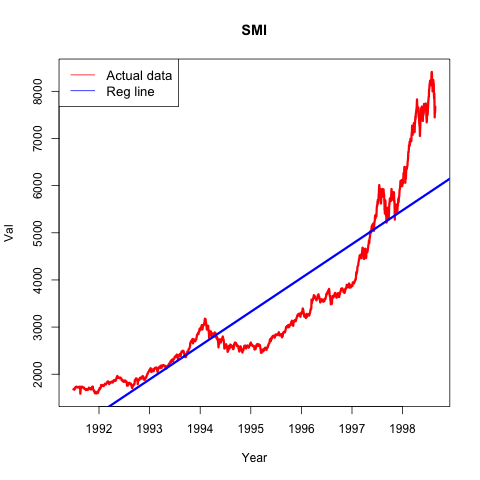
\includegraphics[width = 0.4\linewidth]{data/stockmark_reg_SMI.png} \\
            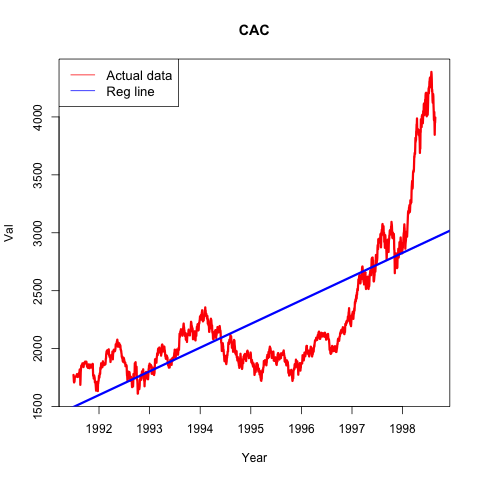
\includegraphics[width = 0.4\linewidth]{data/stockmark_reg_CAC.png} & 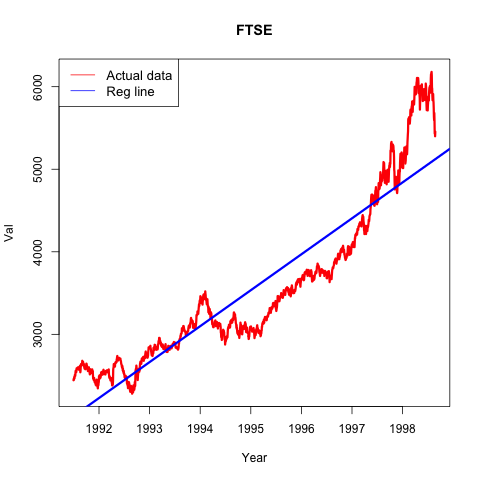
\includegraphics[width = 0.4\linewidth]{data/stockmark_reg_FTSE.png}
        \end{tabular}
        \vspace{-0.5cm}
        \caption{Линии регрессии для каждой биржи}
    \end{figure}

    В целях наглядности для оценки динамики изменения был построен график линий регрессии для всех бирж (Рис. 4).

    \begin{figure}[H]
        \centering
        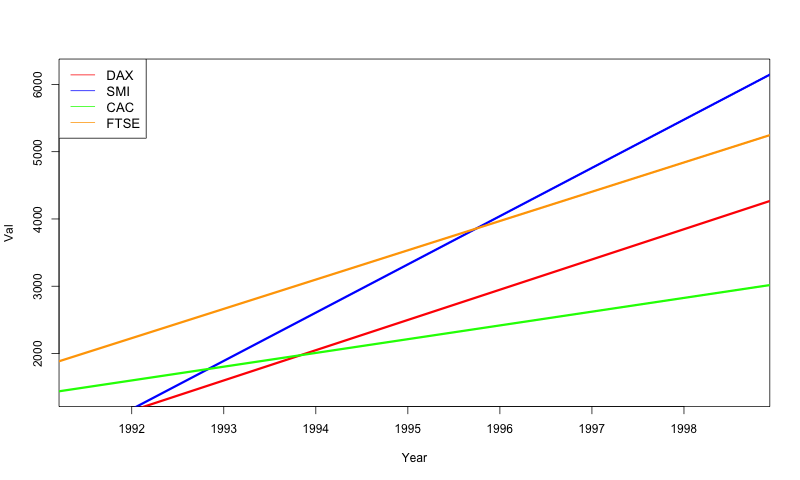
\includegraphics[width = 0.9\linewidth]{data/stockmark_reg_lines.png}
        \caption{Линии регрессии для набора данных <<EuStockMarkets>>}
    \end{figure}

    Основываясь на полученных данных можно сделать вывод, что биржа <<Switzerland SMI>> имеет наибольшую динамику.

    \section{Набор данных <<JohnsonJohnson>>}

    Для того, чтобы изучить набор данных были построенные кривые изменения во времени для всех кварталов (Рис. 5).

    \begin{figure}[H]
        \centering
        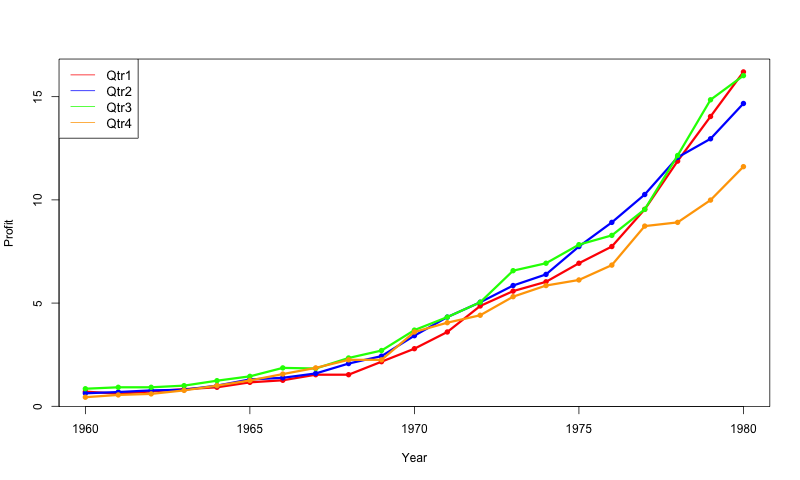
\includegraphics[width = 0.8\linewidth]{data/JnJ_qtr.png}
        \vspace{-0.6cm}
        \caption{Набор данных <<JohnsonJohnson>>}
    \end{figure}
    \vspace{-0.6cm}
    Были построены модели линейной регрессии для каждого из кварталов по отдельности (Рис. 6).
    \vspace{-0.6cm}
    \begin{figure}[H]
        \centering
        \begin{tabular}{c c}
            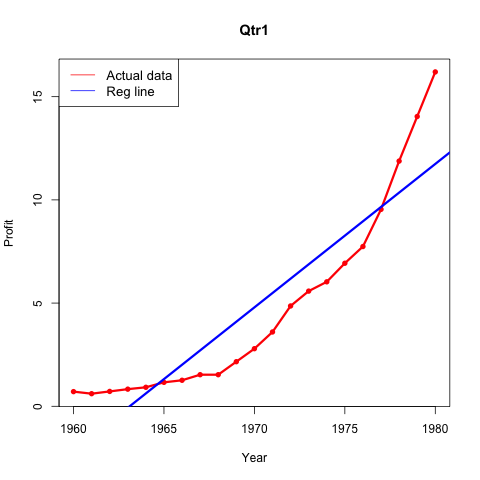
\includegraphics[width = 0.4\linewidth]{data/JnJ_reg_line_qtr1.png} & 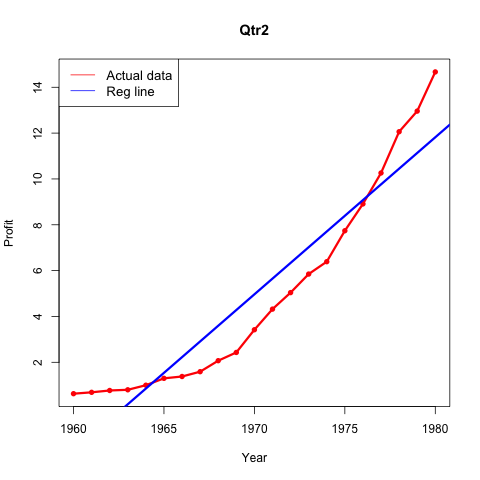
\includegraphics[width = 0.4\linewidth]{data/JnJ_reg_line_qtr2.png} \\
            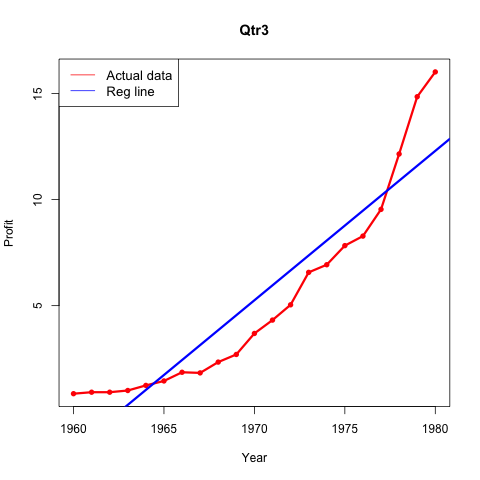
\includegraphics[width = 0.4\linewidth]{data/JnJ_reg_line_qtr3.png} & 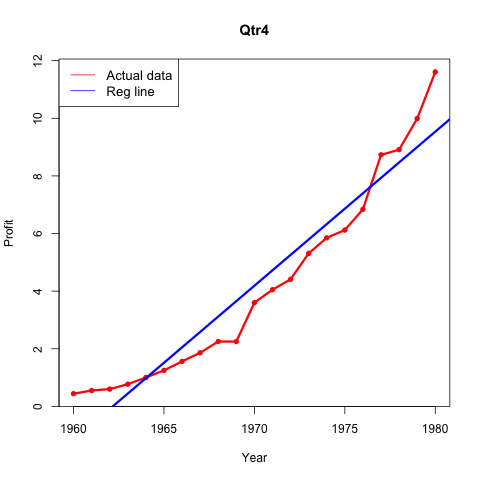
\includegraphics[width = 0.4\linewidth]{data/JnJ_reg_line_qtr4.png}
        \end{tabular}
        \vspace{-0.5cm}
        \caption{Линии регрессии для каждого квартала}
    \end{figure}

    Также была построена линейная регрессия для всех кварталов вместе (Рис. 7)

    \begin{figure}[H]
        \centering
        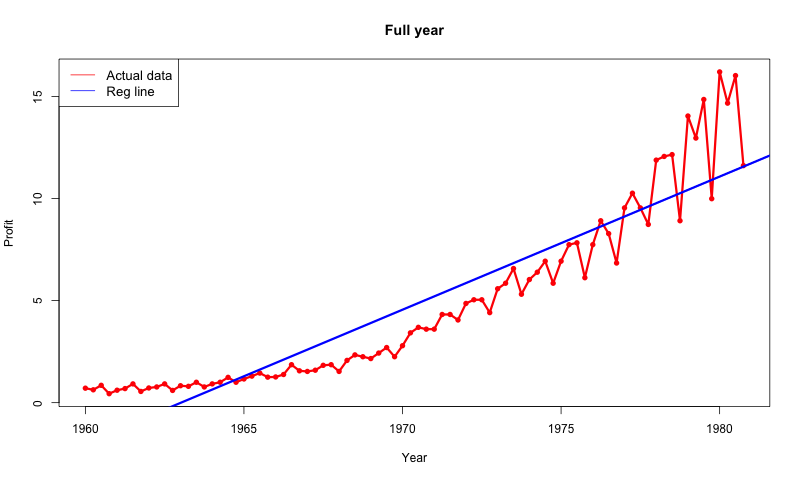
\includegraphics[width = 0.9\linewidth]{data/JnJ_reg_line_full.png}
        \caption{Линейная регрессия для всех кварталов вместе}
    \end{figure}

    В целях наглядности для оценки динамики изменения был построен график линий регрессии для всех кварталов по отдельности (Рис. 8).

    \begin{figure}[H]
        \centering
        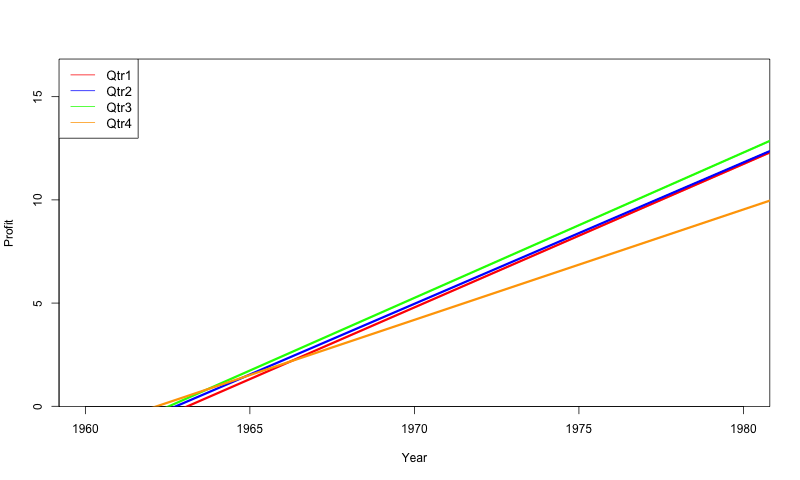
\includegraphics[width = 0.9\linewidth]{data/JnJ_reg_lines.png}
        \caption{Линии регрессии для набора данных <<JohnsonJohnson>>}
    \end{figure}

    Основываясь на полученных данных можно сделать вывод, что наибольшая динамика в 3ем квартале.

    Также в рамках задания был сделан прогноз по прибыли в 2016 году во всех кварталах и в среднем по году (Листинг 6)

    \begin{lstlisting}[style = TEXTstyle, caption = Прогноз на 2016 год]
2016 full:
Min. 1st Qu.  Median    Mean 3rd Qu.    Max.
34.56   34.68   34.80   34.80   34.92   35.05
2016 qtr1:
Min. 1st Qu.  Median    Mean 3rd Qu.    Max.
36.76   36.76   36.76   36.76   36.76   36.76
2016 qtr2:
Min. 1st Qu.  Median    Mean 3rd Qu.    Max.
36.49   36.49   36.49   36.49   36.49   36.49
2016 qtr3:
Min. 1st Qu.  Median    Mean 3rd Qu.    Max.
37.65   37.65   37.65   37.65   37.65   37.65
2016 qtr4:
Min. 1st Qu.  Median    Mean 3rd Qu.    Max.
28.79   28.79   28.79   28.79   28.79   28.79
    \end{lstlisting}

    \section{Набор данных <<sunspot.year>>}
    Для изучения набора данных был построен график (Рис. 9)

    \begin{figure}[H]
        \centering
        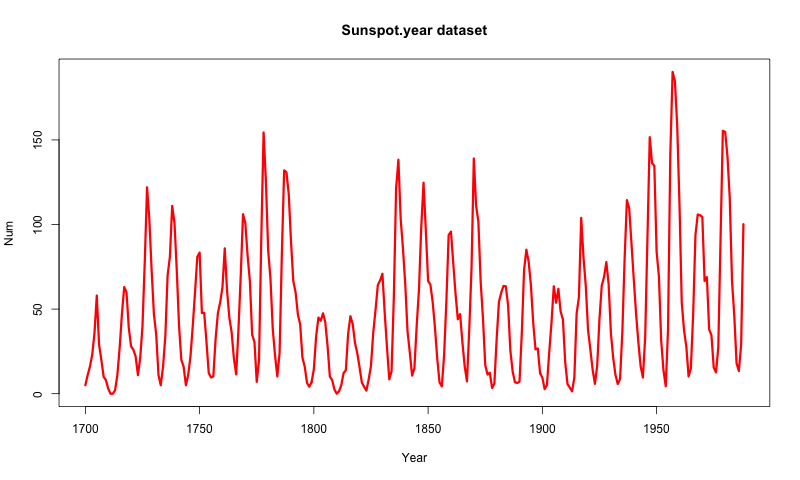
\includegraphics[width = 0.9\linewidth]{data/sunspotyear_data.png}
        \caption{Набор данных <<sunspot.year>>}
    \end{figure}

    Была построенная линейная регрессия (Рис. 10)

    \begin{figure}[H]
        \centering
        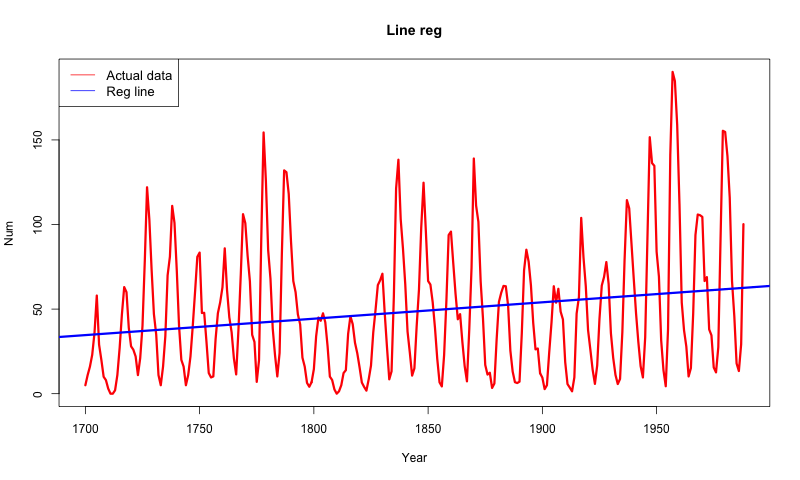
\includegraphics[width = 0.9\linewidth]{data/sunspotyear_reg.png}
        \caption{Линейная регрессия для набора данных <<sunspot.year>>}
    \end{figure}

    \section{Набор данных <<UKgas>>}

    Для того, чтобы изучить набор данных были построенные кривые изменения во времени для всех кварталов (Рис. 11).

    \begin{figure}[H]
        \centering
        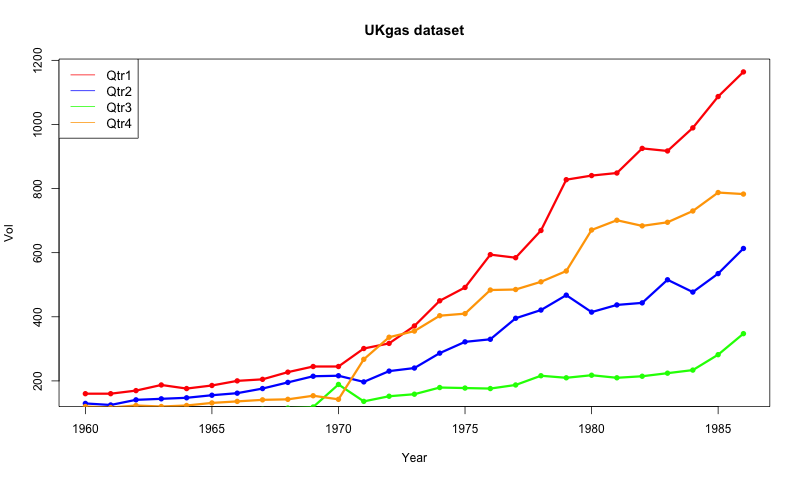
\includegraphics[width = 0.8\linewidth]{data/UKgas_qtr.png}
        \caption{Набор данных <<UKgas>>}
    \end{figure}
    Были построены модели линейной регрессии для каждого из кварталов по отдельности (Рис. 12).
    \begin{figure}[H]
        \centering
        \begin{tabular}{c c}
            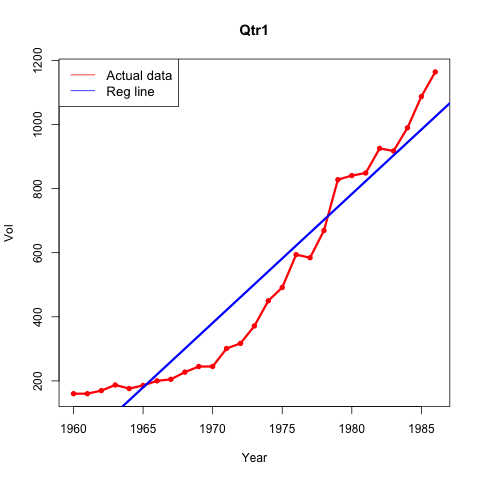
\includegraphics[width = 0.4\linewidth]{data/UKgas_reg_line_qtr1.png} & 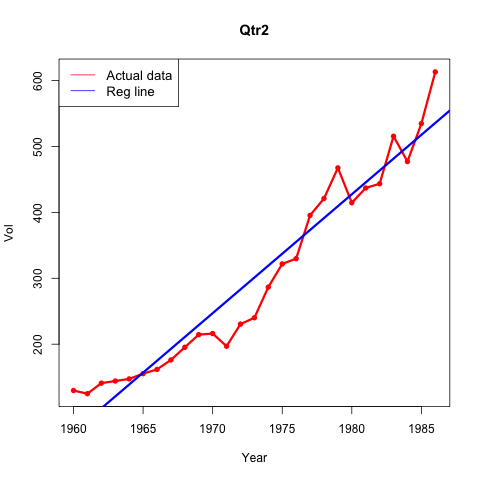
\includegraphics[width = 0.4\linewidth]{data/UKgas_reg_line_qtr2.png} \\
            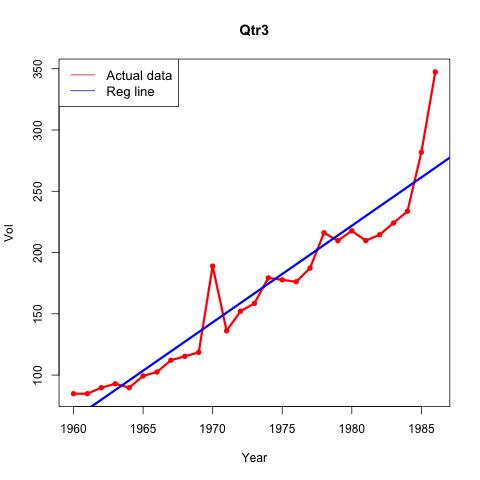
\includegraphics[width = 0.4\linewidth]{data/UKgas_reg_line_qtr3.png} & 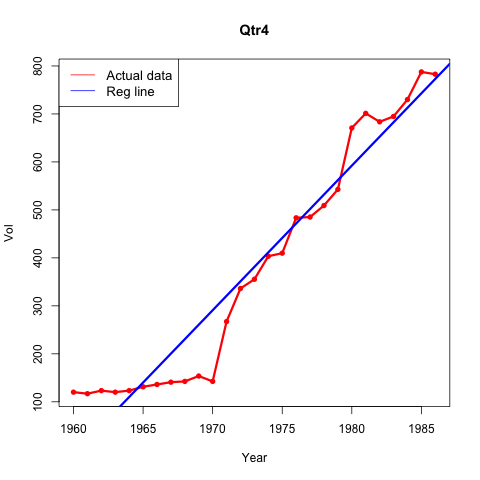
\includegraphics[width = 0.4\linewidth]{data/UKgas_reg_line_qtr4.png}
        \end{tabular}
        \vspace{-0.5cm}
        \caption{Линии регрессии для каждого квартала}
    \end{figure}
    \vspace{-0.4cm}
    Также была построена линейная регрессия для всех кварталов вместе (Рис. 13)
    \vspace{-0.4cm}
    \begin{figure}[H]
        \centering
        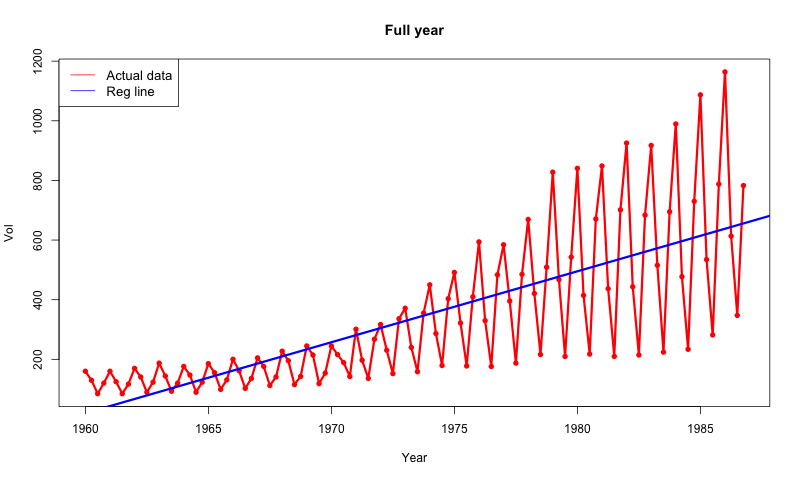
\includegraphics[width = 0.8\linewidth]{data/UKgas_reg_line_full.png}
        \vspace{-0.5cm}
        \caption{Линейная регрессия для всех кварталов вместе}
    \end{figure}

    В целях наглядности для оценки динамики изменения был построен график линий регрессии для всех кварталов по отдельности (Рис. 14).

    \begin{figure}[H]
        \centering
        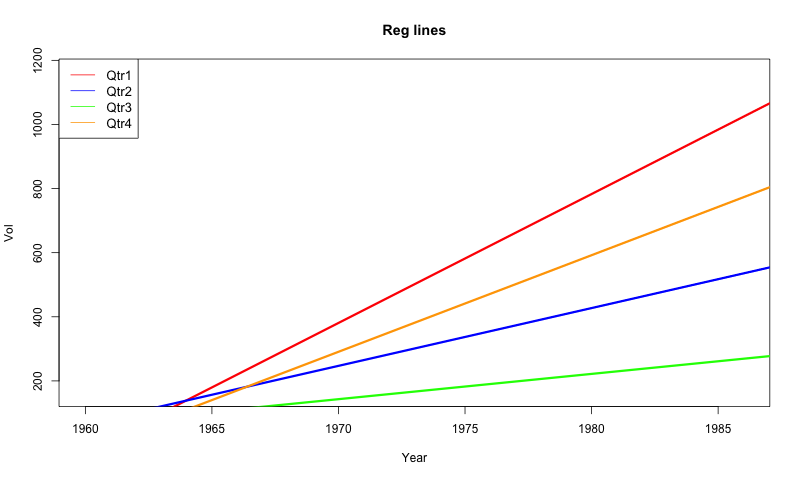
\includegraphics[width = 0.9\linewidth]{data/UKgas_reg_lines.png}
        \caption{Линии регрессии для набора данных <<UKgas>>}
    \end{figure}

    Основываясь на полученных данных можно сделать вывод, что наибольшая динамика в 1ом квартале, а наименьшая в 3ем.

    Также в рамках задания был сделан прогноз по объему газа на 2016 год во всех кварталах и в среднем по году (Листинг 6)
    \vspace{-0.1cm}
    \begin{lstlisting}[style = TEXTstyle, caption = Прогноз на 2016 год]
2016 full:
Min. 1st Qu.  Median    Mean 3rd Qu.    Max.
1352    1356    1361    1361    1365    1369
2016 qtr1:
Min. 1st Qu.  Median    Mean 3rd Qu.    Max.
2231    2231    2231    2231    2231    2231
2016 qtr2:
Min. 1st Qu.  Median    Mean 3rd Qu.    Max.
1077    1077    1077    1077    1077    1077
2016 qtr3:
Min. 1st Qu.  Median    Mean 3rd Qu.    Max.
505.9   505.9   505.9   505.9   505.9   505.9
2016 qtr4:
Min. 1st Qu.  Median    Mean 3rd Qu.    Max.
1677    1677    1677    1677    1677    1677
    \end{lstlisting}

    \section{Набор данных <<cars>>}
    Для наглядности набор данных был визулизирован (Рис. 15).

    \begin{figure}[H]
        \centering
        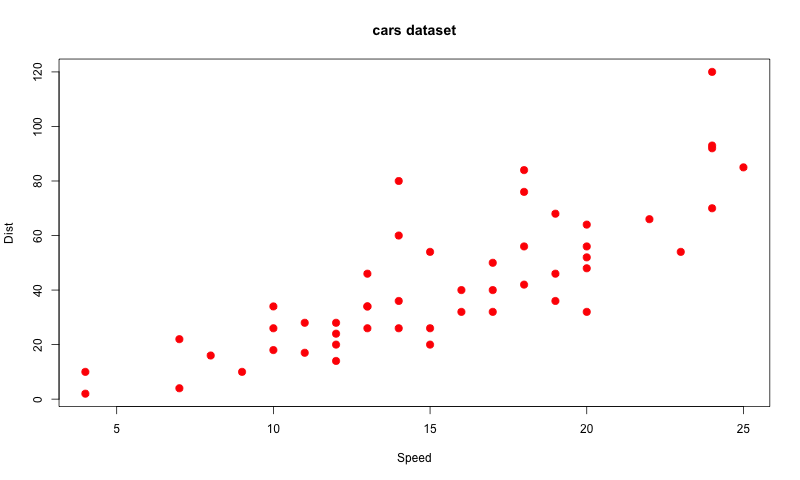
\includegraphics[width = 0.9\linewidth]{data/cars_data.png}
        \caption{Набор данных<<cars>>}
    \end{figure}

    Была построена линейная регрессионная модель (Рис. 16).

    \begin{figure}[H]
        \centering
        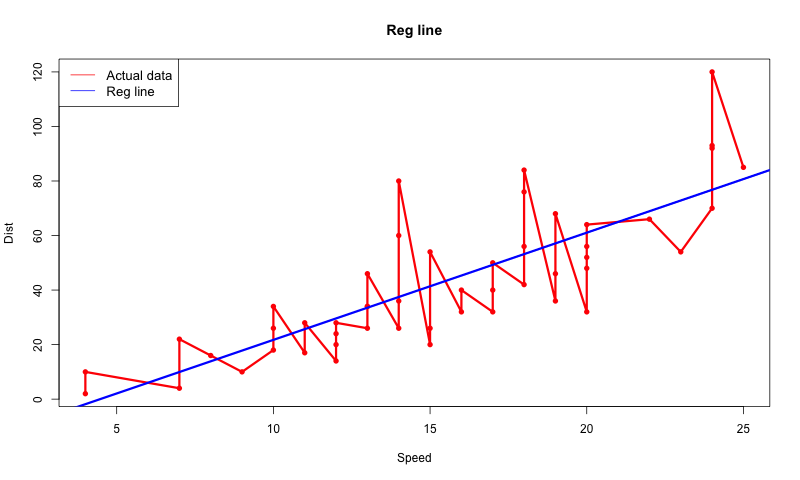
\includegraphics[width = 0.9\linewidth]{data/cars_reg_line.png}
        \caption{Регрессионная модель для набора данных <<cars>>}
    \end{figure}

    Также был предсказан тормозной путь при скорости 40 миль в час (Листинг 8).

    \begin{lstlisting}[style = TEXTstyle, caption = Предсказание тормозного пути при скорости 40 м/ч]
speed = 40:
Min. 1st Qu.  Median    Mean 3rd Qu.    Max.
139.7   139.7   139.7   139.7   139.7   139.7
    \end{lstlisting}

\end{document}
